\chapter{Background and Literature Review}
\label{chapter:background} 

Human Detection can be conducted using a varierty of methods, such as, Passive Infrared Sensors (PIR's), Presure sensors, Thermal Imaging, Infrared Cameras, Video Cameras, Carbon dioxide concentration, and Range Finders like RADAR, Sonar and Lidar.

\section{Previous Study}
\subsection{Cameras and Imagers}
In comparison to other sensors, Cameras are relatively affordable, easy to access, provides reliable, high resolution and easy to interpret information. This is why computer vision has always been a hot topic of the industry.
\\

Sarkar, A, et al.~\cite{sarkar2008integrated} used a high dynamic range CMOS video camera sensors for occupancy sensing and other functionalities like daylight estimation and lighting control. The sensors provides luminance along with the color information. The sensor has the capability of detecting small movements several feet away from the camera as long as it has an adequate resolution. However the system has some feasibility issues like occupancy detection in a region of total darkness. Also the system can not act as a standalone system, it needs to be setup with a workstation.

Shih, Huang-Chia.~\cite{shih2014robust} addressed to the problem of occupancy detection and people  tracking using image-based depth sensor and a programmable pan-tilt-zoom (PTZ) camera.
The system detects the movement even under the the dim lighting scenarios. The system uses -support Vector Machine (SVM) which is a non parametric Machine Learning algorithm. The depth image sensor enables the countour information of the occupant for better activity recognition. The system combines a vision based and sensor based cameras, in order to fill the gap between the subjective sensing of people and system control parameters. 
However this approach is not suitable for working spaces as people might not be comfortable with surveillance cameras mounted near them.
\\

Mikkilineni, Aravind K., et al.~\cite{mikkilineni2019novel} proposed a novel occupancy sensing method which will enable temporal minimization of building energy consumption without privacy concerns, based long-wave infra-red (LWIR) focal-plane arrays (FPAs), or thermal imagers, that detect thermal energy rather than visible light. The solution captures the energy and creates an image whose pixel represents the temperature.  The paper used computer vision based techniques to overcome the accuracy issues suffered by traditional PIR based sensing, especially when the person is still. The paper provides the solution for multiple people tracking and counting at the same time, while addressing to the problem of breach of privacy with normal cameras.
\\

With the advancement of Computer Vision and Deep Neural Networks, occupancy detection using RGB cameras has become quite mundane. However for the purpose of lighting industry, the use of RBG cameras is quite plagued with a lot of loopholes. The first and foremost problem is the privacy infringement. It is against the privacy regulations to record people's activity in the working offices to regulate lighting. The second problem of using RGB cameras is, despite giving the solutions real time, it needs a lot of computational power. Processing the video and then feeding it to a neural network is difficult to be solved using embedded devices. Signal Processing of cameras is more difficult than signals from other sensors.  This is the reason why the cameras or the imagers are not used in the lighting industry which is highly performance driven. 


\subsection{Passive Infrared Sensors (PIR's)}
PIR sensors have been widely used for human detection systems as they are cheap and power consumption is relatively small. The main advantage of PIRs is their unobtrusive and privacy-preserving interaction.
\\

Kim, Sun Ho, et al.~\cite{kim2017improved} studied the use of passive infrared (PIR) sensors along with a door sensor to ensure the accuracy of occupancy detection. The algorithm could detect with an improved occupancy detection accuracy rates of 99.8 \% (when the number of occupants is 1 to 6) and 90.1\% (when the number of occupants is: 1) were achieved.The results of the experiments show that the occupancy detection algorithm along with a door sensor could be used to improve the occupancy detection accuracy rates of
the PIR sensors.
\\
	
Teixeira, Thiago et al.~\cite{teixeira2010survey} provided a survey of the multidisciplinary literature of human-sensing including presence detection.From the presence detection perspective, PIR sensors are often used for binary sensing as they are cheap sensors and have very low power requirements. However, the main
disadvantage of this is that PIRs tend to produce bursty positive detection and a large number of false negative
detection, for example, PIRs cannot sense people who are
standing still.
\\

The use of only PIR sensors for occupancy monitoring does not offer enough savings and depends a lot on the type of the building and its occupancy. Aslam, Javed, et al.~\cite{manzoor2012occupancy} presented a paper using data fusion approach of traditional occupancy monitoring PIR sensor with passive Radio Frequency Identification (RFID).
The users of the experiment are provided with Ultra High Frequency (UHF) tags. The RFID readers which are mounted on the door, detects any tag tag which passes through them.
\\
However from the saving perspective, The time duration for which the maximum number of lights switched on all at the same time, is much less than PIR. Additionally, the time duration for the minimum number of lights switched ON for
this method is longer than using PIRs standalone 
Due to the less reliability in signal propagation that comes with passive RFID technology, an obvious malfunction of this approach comes when a tag is not read.
\\



\subsection{Sensing using Carbon dioxide}


Ansanay-Alex,Guillaume~\cite{ansanay2013estimating} proposes a algorithm to use only indoor carbon dioxide concentrations to provide estimated occupancy profile in office setup. This paper simply used the gradient of the monitored co2 in order to make detection. The method is well functional for arrivals and departures in a closed space. However the results are considerable if the air change rate of the room remain inert for some duration of time, i.e window opening or door opening may lead to wrong  results. These are also rarely used for the control of lighting systems due to their slow response and sensitivity to environmental conditions~\cite{teixeira2010survey}.
\\

Cali, Davide, et al~\cite{cali2015co2} proposed an algorithm to predict the occupancy detection using concentration of carbon dioxide with cheap co2 sensors. The algorithm uses mass balance equation and assumes air to be homogeneous, i.e, the ideal mix of supply and room air. The results of the algorithm provides correct presence profile up to 95.8\%  of the time, whereas for the people
counting, it correctly predicted up to 80.6\%  of the time. The authors of papers used presence patters as inputs of stochastic user models to predict occupancy. 


\subsection{Pressure sensors}
Another approach to predict the occupancy was proposed by Labeodan, Timilehin, et al. ~\cite{labeodan2016experimental} who evaluated the performance of chair sensors using sensing techniques based on strain, vibration and a mechanical-switch for occupancy detection in an office space.
\\
All three sensors are susceptible to the impact force created by users when they move the chair or when they seat in it. All the three type of sensors were prone to false negatives, however only the vibration and strain sensors gave false positives. At the end of the experiment, the mechanical sensors worked best with accuracy of 99\%. The performance of the mechanical-switch was compared to traditional PIRs for the purpose of lighting control. The results demonstrated that the chair sensors performed better than the PIR sensors.


\subsection{Multiple Sensors}

To compensate the drawback of individual single sensor, many researchers have tried assembling multiple sensors into one system in order to achieve better reliability and accuracy.
\\

Dodier, Robert H., et al.~\cite{dodier2006building} proposed an improved detection of building occupancy using multiple independent detectors by applying graphical probability models called belief networks. The multiple sources of information are clubbed together, creating more powerful sensors, such as, carbon dioxide concentration and space relative humidity.
\\



Ekwevugbe, Tobore, et al.  ~\cite{ekwevugbe2012design} described a novel solution for building occupancy detection using sensor fusion model based on an Artifical -intelligence using Adaptive Neuro-Fuzzy Inference System (ANFIS) algorithm. The system monitors climatic variables, energy data and indoor events obtained from a non-domestic building to infer occupancy patterns.
\\
Climate variables include data like indoor and outdoor variables including temperature, humidity, illumination, VOC and CO2 levels.
Energy data includes using existing sub metering
(for electricity), appliance case temperature monitoring, and monitoring of personal computer (PC) temperature.
Indoor data includes variables such as sound data and  PIR data. The resulting occupancy sensor from this research possessed improved reliability that may not be obtained from a single sensor. 

\subsection{Range Finders}
The Range Finders are devices that work by sending the signals towards the objects, and then calculate the distance by observing the timing or the energy of the received signals reflected from those objects. These devices then extract the 2D or 3D snapshots of the environment. It is worth mentioning that in an indoor environment, multiple reflections, scattering and cluttering add considerable noise to their range ~\cite{teixeira2010survey}. This is the reason why the range finders are usually confined to detection in outdoor spaces like Self Driving Cars. 
Based on the medium of propagation, range finders are classified into different classes :SONAR (sound or ultrasound),  RADAR (radio waves), LIDAR
(light), LADAR (laser).

Among all of the range finders, laser based ranging (LADAR) is least sensitive to multiple reflections, scattering and cluttering. Arras, Kai O., et al.~\cite{arras2007using} presented a paper for the detection and tracking of people with LADAR (laser) range finders. The authors of the papers used supervised learning technique to create a classifier for detection of humans. Unlike vision sensors, LADARs provide a large field of view (FOV) and is almost unaffected by other conditions. The sensors are placed very close to the ground and extract the readings from the legs of the people. A 2D range image is created out of the received signals. The common approach is to extract legs by detecting moving blobs. The experiment obtained detection rates of over 90\%. However the problem still remains of the false negatives. LADARs are still not a reliable solution to be deployed as a standalone. Usually they are paired up cameras for the gaming industry. But they remain less efficient for working premises.
\\

Premebida et al.~\cite{teixeira2010survey} discusses outdoor presence detection like pedestrian detection using exclusively LIDAR based features.


----complete this-------
\\

RADAR is one of the most prominent range finder used for occupancy detection. It can give accurate results in all types of luminance scenarios and all weather conditions.
G\"{u}rb\"{u}z, S. Z., et al.~\cite{gurbuz2007detection} targeted the problem of human target detection using synthetic aperture RADAR (SAR). The human spectrograms are used for the detection as the spectrograms for humans are unique is comparison to other objects. Simulations show that spectrograms can detect and identify human targets in low noise. However this approach works only if the target is close to the antenna and signal to noise ratio (SNR) is high. In an indoor environment where the SNR is high, it is very difficult to provide reliable estimation using this method.
\\

Apart from the most common motion sensors i.e. PIRs, other sensors called Doppler shift sensors also exist. Doppler shift means the apparent shift in the frequency of the radial component of the velocity of the object.
Geisheimer et al.~\cite{geisheimer2002high} presented a high resolution Doppler model for the walking human using Continuous Wave (CW) RADAR. The outputs of the RADAR were compared with infrared motion capture system to create the theoretical Doppler signal for walking human. The experiment succeed in unlocking information from the RADAR gait signature, which can be useful in occupancy detection. However the experiment was confined to only standing humans. Further research is required in order to create different signatures for different postures. 
\\

In ~\cite{zhou2006detection}, Zhou et al. used a system which analysed the Doppler RADAR signal of the heartbeat to detect people occupancy in the room. A complex signal processing is used to process these weak signals. Due to Doppler effect, the periodic reflected signals from the chest, gets a phase shift which is proportional to the velocity. The conclusion of the experiment was that less than 2 persons in the room could easily be detected using single antenna of the receiver. To count more people, more antennas are required. 
\\

The ability of the RADARs to penetrate objects like wall, make them less likely to be used for occupancy detection inside the room. For instance Falconer, D. G., et al.~\cite{falconer2000robot} demonstrated a robot mounted motion detection RADAR which is suitable for operations even through the wall( gypsum board walls or hardwood walls). Time domain and frequency domain signals are captured to detect not only the human occupancy but also human's particular activity like resting, walking, talking.



\\

\section{RADAR technology}
RAdio Detection And Ranging is an electromagnetic range finder device that observed the echoed signals by their time delays.  The RADAR can operate in radio or the microwave domain. 
It for various applications on ground, on sea and in space. The applications of RADARs are controlling the Air Traffic, Ship safety, Sensing the remote places, Military applications etc~\cite{RADAR}.

As shown by Figure~\ref{fig:basic_principle}, the RADAR consists of a \textbf{Transmitter} which is used to send the signals, a \textbf{Receiver} which is used to receive the echoed signals.
The received signals are then analysed to process the range, the velocity of the targeted object. 

\begin{figure}[ht]
  \begin{center}
    % below the size of the figure has been reduced for example
    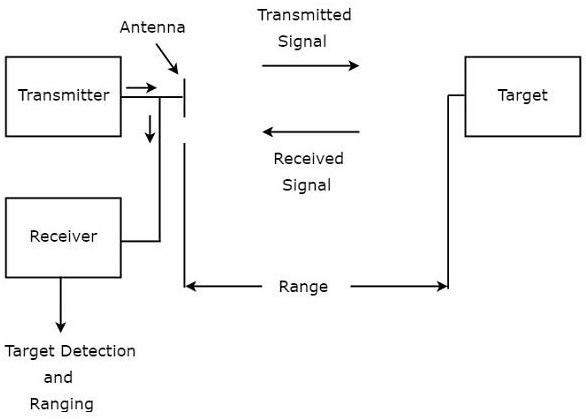
\includegraphics[width=0.80\textwidth]{Master's thesis/images/basic_principal.jpg} 
    \caption{The basic principle of RADAR.}
    \label{fig:basic_principle}
  \end{center}
\end{figure}

\subsection{Types of RADARs}

On a broad level, the RADARs can be divided into \begin{enumerate}
    \item \textbf{Pulse RADAR}
    
    In Pulse RADAR, the RADAR operates with Pulse signals. The RADAR sends the signals for a pulse of duration and then waits to receive the signals. The Pulse RADAR is further classified into Basic Pulse RADAR and Moving Target Indicator RADAR (MTI)
    \begin{enumerate}
    \item \textbf{Basic Pulse RADAR}
    
    It uses single antenna for both sending and receiving signals.  The antenna transmits signals after every clock pulse. This type of RADAR can only detect stationary objects.
    
    \item \textbf{Moving Target Indicator RADAR (MTI)}
    
    This type of RADAR uses pulse signals to compute even the non stationary objects. This uses Doppler effect to distinguish the non stationary object with stationary object.  
    
\end{enumerate}
    \item \textbf{Continuous Wave RADARs}
    
    On the other hand,  Continuous Wave RADARs sends continuous signals in order to detect objects. Both stationary and non-stationary objects can be detected using Continuous wave RADARs. Continuous wave RADARs are further divided into Unmodulated Continuous Wave RADAR  and Frequency Modulated Continuous Wave RADAR(FMCW).
    \begin{enumerate}

    \item \textbf{Unmodulated Continuous Wave RADAR}
   
    This type of RADAR detects non stationary objects using continuous wave signals. It is also called Continuous Wave Doppler RADAR. It is worth noticing that the frequency of the continuous signal remains unchanged over time.
    
    \item \textbf{Frequency Modulated Continuous Wave RADAR (FMCW)}
    
    This is the most advanced type of RADAR which can be used for detecting the both the stationary and non stationary objects.An FMCW RADAR requires two antennas- one for transmitting and the other one for receiving. The distance and velocity of the objects can be easily computed using Fourier transformations (FFT) of the received signals. More detailed explanation about FMCW is provided in the following section. 
\end{enumerate}
\end{enumerate} 







\subsection{Frequency Modulated Continuous Wave RADAR (FMCW)}

Continuous Wave Radar are popular because of low power consumption and simple radio architecture. Also,these type of Radars cancel out clutter noise by proper adjustment. The main advantages of the FMCW remains good range resolution, resistance to interception, simple solid-state transmitters. FMCW method performs the velocity and range measurement efficiently and therefore it is a good solution for lighting industry~\cite{arai2000life}~\cite{li2006experiment}.


FMCW generates a linearly increasing frequency signal viz., sawtooth or sinusoidal wave using a synthesizer. The generated signal is then transmitted using one or more antennas.
Each signal is called \textbf{chirp/sweep}. A chirp is a signal whose frequency increase linearly with time ~\cite{rao_2017}. A chirp can be characterized by the four features broadly-

\begin{itemize}
    \item start frequency which is generally called carrier frequency and denoted by \(f_{c}\),
    \item a chirp bandwidth(\(B\)), which is the difference between the maximum reachable frequency  \(f_{c} + B \)  and the carrier frequency \(f_{c}\).
    \item the sweep time(\(t_{p}\)), which is the duration for which an FMCW sends one chirp,
    \item The slope(\(k= B/t_{p}\)), of the chirp which is defined as rate at which the chirp ramps up. It is the ratio between the chirp bandwidth and the sweep time.
    
 \begin{figure}[ht]
  \begin{center}
    % below the size of the figure has been reduced for example
    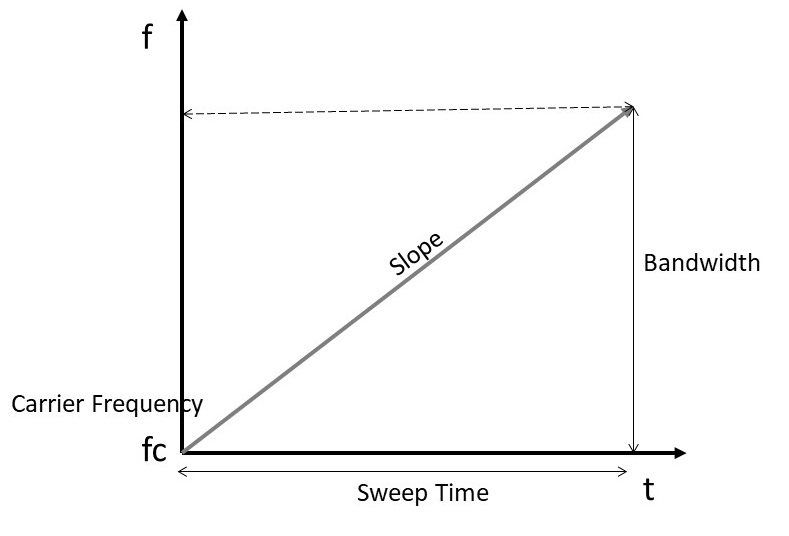
\includegraphics[width=0.60\textwidth]{Master's thesis/images/sweep.jpg} 
    \caption{A basic Chirp/Sweep signal}
    \label{fig:sweep}
  \end{center}
\end{figure}   
\end{itemize}

Therefore, the frequency of the signal \(f_{t}\) at any time \(t\), with carrier frequency \(f_{c}\) , amplitude \(A_{t}\), slope \(t\), is given by the following expression

\[f_{t}= A_{t}cos[2\pi(f_{c}t + \frac{k}{2}t^2)]\]

The transmitted signal TX is transmitted through the transmitter antenna. The TX signal strikes the surface of the object and gets reflected back. The receiver of the FMCW receives this reflected signal RX via its receiving antenna. RX signal is just the same TX signal but delayed.
To compute the range, velocity or phase of the object, the most important factor to measure is the \textbf{Baseband signal} with frequency IF known as \textbf{Intermediate Frequency (IF)}. The frequency of the Baseband signal is the difference of the instantaneous frequency of the TX-chirp and RX-chirp. It is to be noted that for a stationary object, irrespective of when the  chirp was transmitted, this IF signal will remain same, as this IF signal is proportional to the delay time which is proportional to the distance of the object from Radar.

Figure ~\ref{fig:IF} explains the IF signal in the mathematical way. 
 \begin{figure}[ht]
  \begin{center}
    % below the size of the figure has been reduced for example
    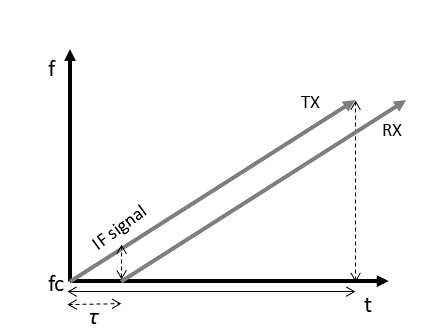
\includegraphics[width=0.60\textwidth]{Master's thesis/images/IFSignal.png} 
    \caption{A Baseband signal with Intermediate frequency IF}
    \label{fig:IF}
  \end{center}
\end{figure}   

 \begin{figure}[ht]
  \begin{center}
    % below the size of the figure has been reduced for example
    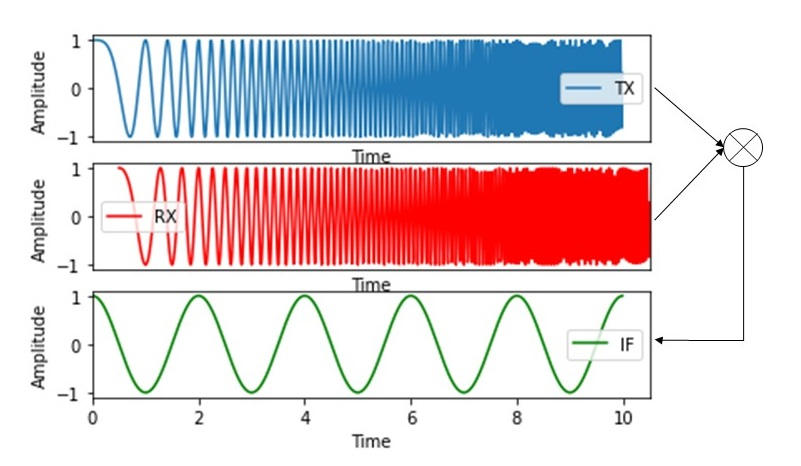
\includegraphics[width=0.80\textwidth]{Master's thesis/images/mixer.jpg} 
    \caption{A resultant IF signal from Mixer}
    \label{fig:Mixer}
  \end{center}
\end{figure}  

Figure ~\ref{fig:fmcw} explains in detail on how this Baseband signal is produced. 
The \textbf{Frequency Modulator} produces a modulated frequency signal TX which is transmitted using \textbf{Transmitter}. The \textbf{Local Oscillator} produces a signal having Radio Frequency \(f_{rf}\). The output of the Local Oscillator is then feeded to a mixer along with the output of the Transmitter. The \textbf{Mixer} computes then sum and the difference of the Transmitted frequency and the RF signal from Local Oscillator. A low pass filter then only allows the lower frequency to be passed i.e. only the difference of the Transmitter and the RF signal \(f_o(t) - f_{rf}\) is allowed ~\cite{tutorialspoint}. 

Another \textbf{Mixer}, is feeded the received signal from the receiving antenna \(f_r\) and the output of the low pass filter. It is worth mentioning that the received signal RX is just a delayed version of the transmitted signal TX. It then computes the sum and the difference of these signals again, i.e. \(f_r\) + \(f_o(t) - f_{rf}\), \(f_r\) - (\(f_o(t) - f_{rf}\))~\cite{tutorialspoint}. An \textbf{Amplifier} amplified the differenced output of the Mixer, i.e. only \(f_r\) - \(f_o(t) + f_{rf}\) is amplified. The \textbf{Balance Detector} which is connected to both the Amplifier and the Local Oscillator computes the difference of the both input signals, hence generating a signal of frequency \(f_r - f_o(t)\). 
This output is then inputted to \textbf{Low Frequency Amplifier} which amplifies the input frequency. This resultant signal is then called the Baseband signal ~\cite{tutorialspoint}. 

 \begin{figure}[ht]
  \begin{center}
    % below the size of the figure has been reduced for example
    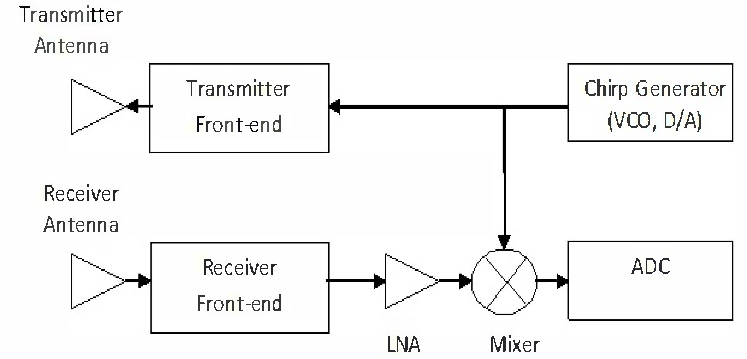
\includegraphics[width=0.80\textwidth]{Master's thesis/images/fmcw.png} 
    \caption{Block Diagram for FMCW}
    \label{fig:fmcw}
  \end{center}
\end{figure}   

In order to understand the functionality of FMCW in better detail, we will divide the topic into 3 parts.
\begin{itemize}
    \item Part 1: Evaluation of the range of the target object.
    \item Part 2: Evaluation of velocity of the target object.
    \item Part 3: Evaluation of phase of the target object.
\end{itemize}
\\

\subsection{Signal Processing for FMCW}
The Baseband signal is constructed by the Radar when an object reflects the signals. However in a real scenario, there are multiple objects in the scene resulting in multiple Baseband signals. Therefore Radar receives combination of these Baseband signals. To differentiate different objects, Radar should be able to differentiate between different signals. To do so, Radar uses Fourier Transformations. A brief summary of Fourier Transformations is provided in the following subsection.


\subsubsection{Fourier Transformation} \label{sec:FT}
According to ~\cite{FT}
\say{Fourier transform (FT) is a mathematical transform that decomposes functions depending on space or time into functions depending on spatial or temporal frequency.}
Specific to FMCW, Fourier Transform is used to convert a time domain signal into the frequency domain. 
Consider a frequency signal in the form -  
\begin{equation}\label{eq:eq1}
A_{t}= ASin[2\pi ft + \phi]
\end{equation}
Let's suppose A =2, t= 1sec, \(\phi\) = 0 and f = 4.
\\
Therefore, the eq ~\ref{eq:eq1} becomes
\begin{equation}
A_{t}= 2Sin[8\pi]    
\end{equation}

The Fourier Transformation of this signal, returns a frequency-amplitude domain signal, with a peak at \textbf{4} as the frequency of the signal was 4.

 \begin{figure}[ht]
  \begin{center}
    % below the size of the figure has been reduced for example
    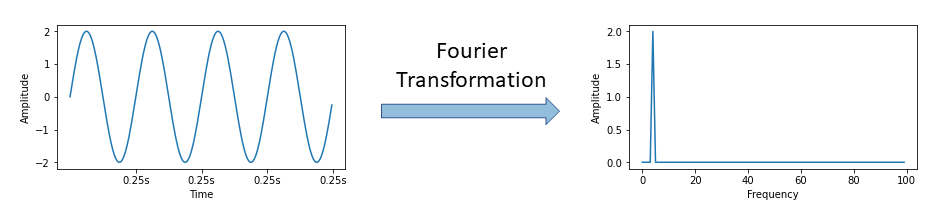
\includegraphics[width=1\textwidth, height = 3.5cm ]{Master's thesis/images/fft.png} 
    \caption{Fourier Transformation of a constant frequency signal}
    \label{fig:fft}
  \end{center}
\end{figure}  

However, in a real time scenario, signals are not continuous, rather discrete. Therefore for discrete signals, Discrete Fourier Transform (DFT) is commonly used. The resolution limit is determined by the number of input samples.
The output of the DFT has the same size as input. For a device like Radar where the frequency of the signal is usually in GHz, the sampling index is huge, therefore the number of outputs of DFT will be huge. Increasing the number of inputs, increased the computation power by $O[N^2]$.
\\

Therefore, to the computations less complex, the number of samples are chosen as a power of $2^N$ which enables to use Fast Fourier Transform (FFT) instead of DFT. The complexity of FFT is $O[NlogN]$ instead of $O[N^2]$. FFT can be used either by increasing the sampling rate or by appending zeros at the end before performing FFT. Zero padding makes the resolution between two consecutive bins easier.

It is worth mentioning that the resolution of the FFT increases with the length of the observation period. In general, an observation window if T can separate frequency components that are separated by more than $\frac{1}{T}$ Hz~\cite{rao_2017}.
%windowing%


\subsubsection{Range Evaluation for Stationary targets}\label{sec:rangeEval}

Consider an object as distance $d$ from the FMCW Radar. From ~\ref{fig:IF}, we can clearly say that the frequency of the IF signal is 
\begin{equation}\label{eq:range}
    f_{\tau}= k\tau
\end{equation}
where k is the slope of the chirp, $\tau$ is the delay in the RX signal.
But 
\begin{equation}
    Time = Distance*Speed
\end{equation}
Therefore, substituting Distance = 2d ( To and fro distance covered by the signal from Radar) and Speed = c (speed of light) into eq ~\ref{eq:range}, we get:
\begin{equation}\label{eq:range_eq}
f_{\tau}= k\frac{2d}{c}   
\end{equation}

Eq ~\ref{eq:range_eq} indicates the Intermediate frequency of the Baseband signal obtained from an object placed at a distance d.
\\


In a real scenario, an FMCW receives a signal which is a combination of different Intermediate Frequencies. These IF signals are produced by objects placed at different ranges. From Eq~\ref{eq:range_eq}, it is evident that these IF signals are proportional to the distance d at which the object is placed.
This is where Fourier Transformations discussed in section ~\ref{sec:FT} comes into picture.

To calculate the range of different objects present in the view, the output received by the FMCW Receiver is transformed using FFT. This result is called \textbf{Range FFT} of the received signal RX.

For instance, let's imagine the receiver receives the composite signal as shown in the Fig \ref{fig:comp_fft}. The signal is formed by addition of two different IF signals with frequencies of 4 Hz and 6 Hz, and the amplitude of 2 m and 3 m.
The frequencies and the amplitude of these composite signals can be easily obtained by using FFT on this signal. The plot beneath the composite signals indicates the FFT output on the composite signal.
Therefore, in a real time scenario to obtain a range estimation of all the objects in the frame, it is important to use Range FFT.
 \begin{figure}[ht]
  \begin{center}
    % below the size of the figure has been reduced for example
    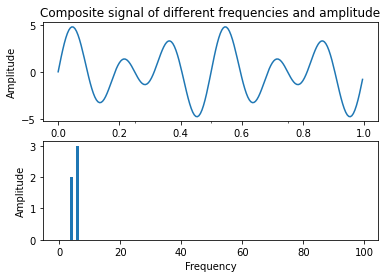
\includegraphics[width=0.6\textwidth]{Master's thesis/images/comp_fft.png} 
    \caption{Fourier Transformation of a composite signal}
    \label{fig:comp_fft}
  \end{center}
\end{figure}  

\textbf{Range Resolution} is defined as the minimum distance that should be there in between two objects to differentiate them for FMCW. As previously explained, in order to differentiate two objects, the frequency difference should be at least 1/T i.e., 
\begin{equation}\label{eq:fgtt}
 \Delta f > \frac{1}{T}  
\end{equation}Consider two objects, placed at a distance of $d_{1}$ and $d_{2}$, from eq~\ref{eq:range_eq}, their respective IF frequencies are given by
 \begin{equation}
   f_{\tau1}= k\frac{2d_{1}}{c}
 \end{equation} 
 
 and
  \begin{equation}
   f_{\tau2}= k\frac{2d_{2}}{c}
 \end{equation} 
 
 Therefore, 
 \begin{equation}\label{eq:deltaf}
     \Delta f = k\frac{2\Delta d}{c}
 \end{equation}
Substituting Eq~\ref{eq:deltaf} in Eq ~\ref{eq:fgtt} and T with the observation period $T_{c}$, we get,
\begin{equation}
  k\frac{2\Delta d}{c} > \frac{1}{T_{c}}  \implies \Delta d > \frac{c}{2kT_{c}} \implies \Delta d > \frac{c}{2B}  
\end{equation}
where $B$ is the Bandwidth of the chip and is equal to $kT_{c}$.

Hence, the Range Resolution ($d_{res}$), depends only on the speed of the light and Bandwidth of the chirp~\cite{rao_2017}, $\therefore$ 

\begin{equation}
   d_{res} = \frac{c}{2B} 
\end{equation}

\textbf{Maximum Range} of the Radar is defined as the distance beyond which FMCW fails to operate. From Eq. ~\ref{eq:range_eq}, substituting $d$ with $d_{max}$, we get \(f_{IF_max} = \frac{k2d_{max}}{c}\) . Replacing $f_{IF_max}$ with $F_{s}$,where $F_{s}$ is the maximum sampling rate of Radar, we have,
\begin{equation}
    d_{max}= \frac{F_{s}c}{2k}
\end{equation}

This means we an increase or decrease the maximum field of view range by changing either maximum sampling rate or the bandwidth.
\begin{itemize}
    \item Keeping Maximum Sampling rate constant $F_{s}$, the Maximum Range of the Radar can be manipulated by changing the Bandwidth.
    \item Similarly,  Keeping Bandwidth constant, the Maximum Range of the Radar can be manipulated by changing the Maximum Sampling Rate $F_{s}$.
\end{itemize}



\subsubsection{Velocity Evaluation for Moving targets}
According to section~\ref{sec:rangeEval}, to separate different objects in the view, Range FFT is applied on the received RX signal. However the question to ask here is "\textit{How can the two objects placed at same radial distance from FMCW can be separated?}"~\cite{rao_2017}. The FFT of the two objects placed at same distance will give peak bins at the same frequency. However doing further signal, this problem can be resolved using the velocities of these object which are at same distance.

To solve this problem, Fourier Transformation comes into the picture. However instead of doing Range FFT, \textbf{Doppler FFT} is used.

Let's go a step further to what is explained in sec ~\ref{sec:FT}. Note that using Euler's formula, any sinusoidal signal in rectangular form can be expressed in the form of complex exponential signal. A Euler's formula is expressed as \(Ae^{j\theta}\), where $A$ is the amplitude of the signal and $\theta$ is the initial phase of the signal. The Fourier transformation of the signals produces a complex signal, i.e, an amplitude value as well as the phaser. 
In the Fig ~\ref{fig:euler}, waves and their corresponding Euler's representations are shown.

 \begin{figure}[ht]
  \begin{center}
    % below the size of the figure has been reduced for example
    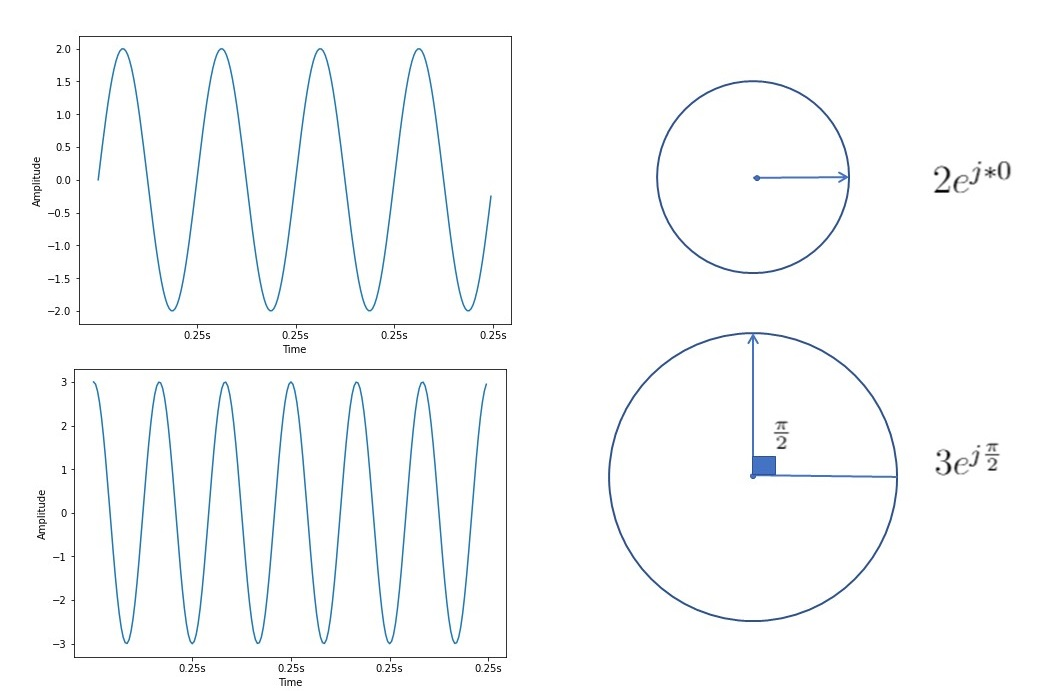
\includegraphics[width=0.8\textwidth]{Master's thesis/images/euler.jpg} 
    \caption{Wave and its Euler representation}
    \label{fig:euler}
  \end{center}
\end{figure}  

Now, consider the Fig ~\ref{fig:Mixer}, what happens if the target object moves by a distance of $\Delta d$. It can be surely said that the frequency of the Baseband signal i.e, Intermediate Frequency will be change by $\frac{2\Delta d}{c}$. This value is close to 0, since $\Delta d$ is very small. However, the initial phase of the IF signal will definitely change, despite the fact that the intermediate frequency is same. Change in $\Delta d$ makes $\Delta\tau$, round trip delay.
Phase $\theta$ of a wave at any time t, can be represented as-
 \begin{equation}
     \theta= 2\pi ft
 \end{equation}
Therefore change in theta with change in time $\Delta t$ is-
 \begin{equation}
     \Delta\theta= 2\pi f\Delta t
 \end{equation}
 For the purpose of simplicity, we represent change in phase i.e, $\delta \theta$ with $\omega$. It is known that, $\Delta t= \frac{2\Delta d}{c}$ and $f= \frac{c}{\lambda},  \therefore$ putting everything together - 
 \begin{equation}\label{eq:theta}
     \omega= \frac{4\pi \Delta d}{\lambda}
 \end{equation} 

This is the change in phase of the IF signal, when an object moves by distance 
\begin{equation}\label{eq:eq1}
A_{t}= ASin[2\pi \frac{k2d}{c}t + \frac{4\pi \Delta d}{\lambda}]
\end{equation}
The phase of the IF signal is very sensitive to to small change in object range ~\cite{rao_2017}.

 \begin{figure}[ht]
  \begin{center}
    % below the size of the figure has been reduced for example
    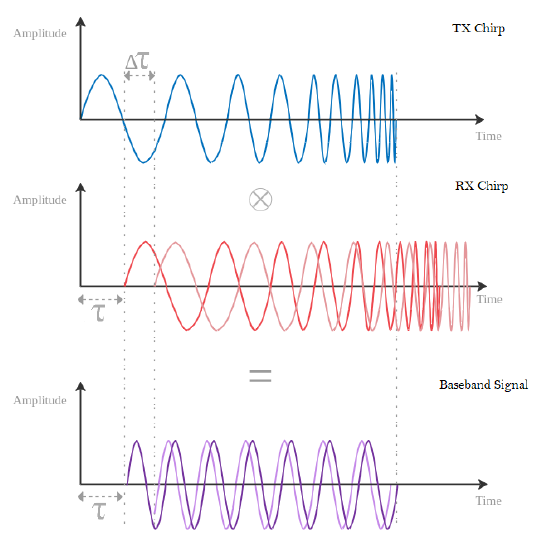
\includegraphics[width=0.6\textwidth]{Master's thesis/images/delay_sweeps.PNG} 
     
    \caption{Two consecutive chirps giving rise to a phase difference}
    \caption*{\textit{Source:} Nilsson, J., Hassbring, L. (2020). Machine Learning for FMCW Radar Interference Mitigation~\cite{nilsson2020machine}.}
    

    \label{fig:delay}
  \end{center}
\end{figure}  

To calculate the velocity of the object, two chirps are transmitted separated by time interval of $T_{c}$.
It is known that $d= vT$ (v is velocity of the target object), From Eq. ~\ref{eq:theta}, substituting $\Delta d$, we get -
\begin{equation}
    \omega= \frac{4\pi v \Delta t}{\lambda}
\end{equation}
Substituting $\Delta t$ with $T_{c}$, which is the time between two consecutive sweeps and reordering, we get-

\begin{equation}
    v= \frac{\lambda \omega}{4\pi T_{c}}
\end{equation}
Therefore, in summary, it can be said that the phase difference obtained from the Fourier transformation of two consecutive chirps, can help in determining the velocity of that object. 

The phase shift between consecutive chirps is the same for any two chirps. This phase shift can be easily calculated by performing FFT on the Range FFT from each chirp. This is called Doppler FFT. The whole process is the called Range-Doppler FFT, i.e, first performing Range FFT on the signals to evaluate the Range and then performing another Doppler FFT on consecutive chirps to obtain the velocities of these objects and then to differentiate them. 
The Range Doppler FFT is done with the help of matrix, with the dimensions N x M where M is the number of chirps and N is the number of samples in each chirp.

A proper visualization of the Range-Doppler FFT process can be seen in Figure ~\ref{fig:range-doppler-FFT}. Every IF signal/Baseband signal have its own phase. Every baseband signal is inserted row wise in a matrix. Every row undergoes a Range FFT operation for Range estimation. This is done in parallel as soon as the FMCW received the RX signals. The result is peak in some columns of the matrix. Once the number of received signals are enough, column wise FFTs are performed for a radial velocity estimation.
 \begin{figure}[ht]
  \begin{center}
    % below the size of the figure has been reduced for example
    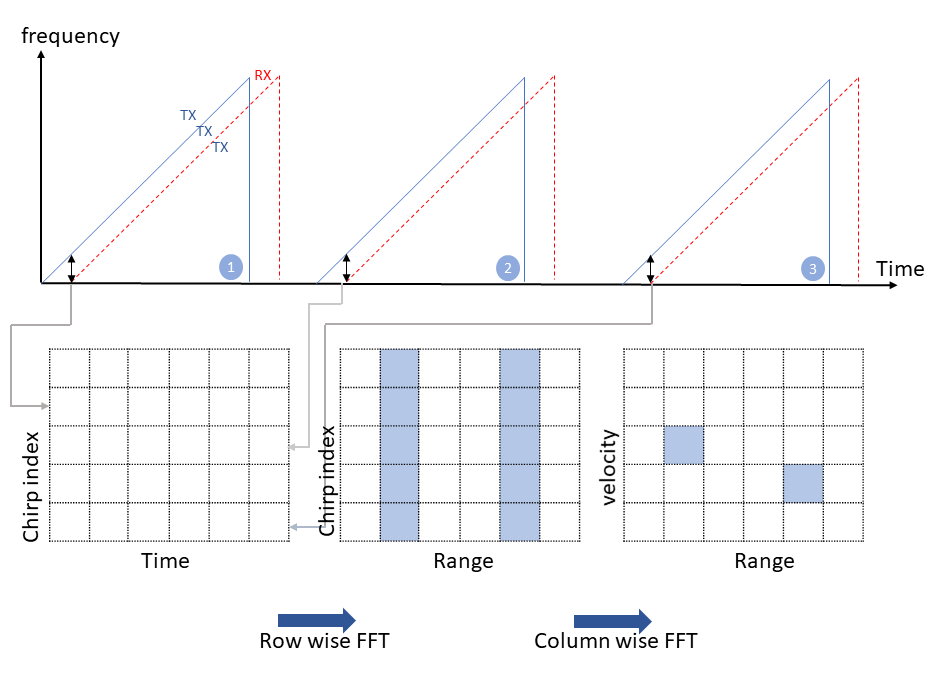
\includegraphics[width=0.7\textwidth]{Master's thesis/images/range_doppler1.png}
    \caption{Range-doppler-FFT}
    \label{fig:range-doppler-FFT}
  \end{center}
\end{figure}  



This results in peaks in different cells of the matrix. These cells corresponds to different objects at different locations from FMCW and moving at a different radial velocity to/from FMCW. The Doppler-FFT change the Range x Chirp index dimension to Range x Velocity. Also, frequency is changed from the range from [0, $2\pi$] to [-$\pi$,$\pi$] in the normalized frequency domain. This makes sure that even the negative velocities are captured.

Therefore in summary, it can be said that for the object at different ranges or the objects at different ranges can be easily detected using Range-Doppler FFT.

\subsubsection{Phase Evaluation for moving targets}

In the previous subsection, the complete process about Range-Doppler FFT was explained. However, now one most case rises up, where the Range-Doppler FFT fails completely. Consider a case where two objects at same radial distance are moving to/from the FMCW at the same radial velocity. The Range-Doppler FFT will give rise to one bin for two different object. So this situation forces us to ask the question
\textit{"How can the two objects placed at same radial distance and moving with same radial velocity from FMCW can be  separated?"}

A very simple answer is to give two eyes to the FMCW. The main advantage of humans having two eyes is to interpret the world in 3D, i.e, humans can perceive the depth of the objects in field of view because eyes are located at different points. So using this analogy, if we use multiple receiving antennas for the FMCW, it will help us solving the problem in question.

An FMCW measures Angle of Arrival(AoA) to resolve this problem. Angle estimation will require a minimum of 2 receiver antennas. Assuming the receiver antennas are placed in close proximity, there ratio of the radial distance from one antenna with other will be close to 1. This means, even if the two antennas in consideration have some Range FFT (as they are almost at same radial distance from the object), there will be a phase change involved. Eq. ~\ref{eq:theta}, shows that an object which made a small change in distance $\Delta d$ in two consecutive sweeps give rise to a phase difference $\Delta \theta$ or $\omega$.
\[\omega= \frac{4\pi \Delta d}{\lambda}\]
Using the same mathematical notation, it can be said that the phase difference between the two antennas will be
\begin{equation}\label{eq:AoA}
\omega= \frac{2\pi \Delta d}{\lambda}    
\end{equation}
Here is the eq.~\ref{eq:AoA}, the equation has a factor of 2 instead of 4 in eq.~\ref{eq:theta}. The difference can be understood by mere intuition. When an object moves by some distance $\Delta d$, the phase difference will brought out by the two and fro signal. Here , in contrast, the phase difference is brought by the distance between the two receiving antennas. This is the reason the eq. has been divided by 2 ~\cite{rao_2017}.
 \begin{figure}[ht]
  \begin{center}
    % below the size of the figure has been reduced for example
    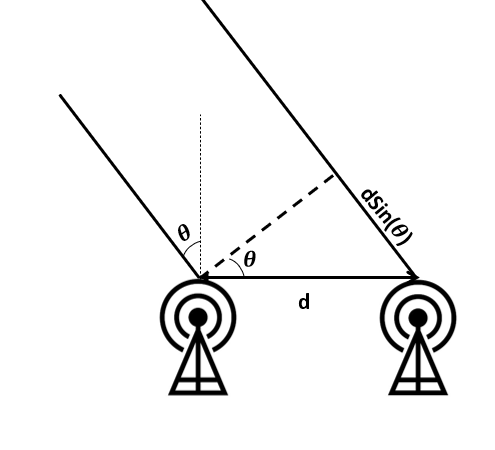
\includegraphics[width=0.3\textwidth]{Master's thesis/images/AoA.PNG} 
    \caption{Angle of arrival in case of two receiver antennas}
    \label{fig:AoA}
  \end{center}
\end{figure}  
Using the geometry of Fig ~\ref{fig:AoA} and using eq.~\ref{eq:AoA}, it can be derived that-
\[\omega= \frac{2\pi dsin(\theta)}{\lambda}\]
Hence, $\theta$ which is the AoA can be derived as-
\begin{equation}
    \theta= sin^{-1}(\frac{\lambda\omega}{2\pi d})
\end{equation}
It is worth mentioning that the maximum phase difference can be more than $\pi$, For phase difference more than $\pi$,it will be impossible to say of the phase difference was actually $\theta$ or $\theta-\pi$.

Now consider the \textbf{figure},it is pretty much evident that the two objects at same radial distance will result in same peaks in the Range-Doppler FFT, however multiple antennas give rise to a phase difference.




If another FFT is applied on these phase differences, this give rise to an FFT sequence which is called \textbf{angle-FFT}. Angle FFT helps in resolving such two objects.


\subsubsection{Micro Doppler}


\subsection{RADAR Specifications}
The RADAR used in this thesis has a carrier frequency of 24 Ghz. The Bandwidth of the frequency is 250 MHz and the sweep time is 1 ms.
S. No.	Specification	Value
1	Carrier Frequency	
2	Bandwidth of 1 sweep	
3	Sweep Time	
4	Min sweep interval	
5	Centre Angle	
6	Max view distance 	14 m
		
\section{Lighting Industry}
\section{Machine Learning Literature Review}




